\newcommand{\erassistant}{ErAssistant~}

\chapter{ПРОБЛЕМАТИКА РАЗРАБОТКИ \\МУЛЬТИСИНХРОННЫХ УСТРОЙСТВ}

В данном разделе будут рассмотрены проблемы и особенности построение устройств


В этом разделе будут описаны проблемы, возникающие в процессе разработки мультисихронного проекта, то есть устройства, в котором имеют место пересечения клоковых доменов или доменов синхрочастоты (CDC).

\section{Домен синхрочастоты}
Домен синхрочастоты представляет собой ту часть проекта, которая тактируется одной или несколькими синхрочастотами, причем все эти синхрочастоты должны иметь постоянные сдвиги фазы. Если в какой-либо части проекта имеется синхрочастота или инвертированная синхрочастота, или синхрочастота, полученная из исходной путем деления на 2, то такая часть проекта считается клоковым доменом с одной синхрочастотой. Если же домены имеют синхрочастоты с переменной фазой и соотношениями времени, то такие домены считают доменами с различными синхрочастотами. 

На Рисунке \ref{fig:clock-domain} показано, что проект имеет единственный домен синхрочастоты, потому что синхрочастота divClk --- есть деленная на два частота генератора синхронизации Clk.

\begin{figure}
	\centering
	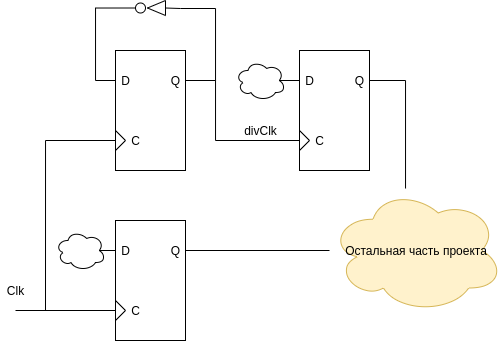
\includegraphics[width=0.6\linewidth]{course-scheme/images/clock-domain}
	\caption{Проект, имеющий единственный домен синхрочастоты}
	\label{fig:clock-domain}
\end{figure}


На Рисунке \ref{fig:multiclock-domain} показано несколько синхрочастот от различных источников. Ту часть проекта, которая управляется этими синхрочастотами, называют доменами синхрочастоты, и сигналы, осуществляющие передачу импульсов между этими асинхронными доменами синхрочастоты, называют путями пересечения домена синхрочастоты. Сигнал DA считают асинхронным сигналом в домене синхрочастоты, так как между генератором синхронизации A (clkA) и генератором синхронизации B (ClkB) не существуют постоянные соотношения фазы и времени.

\begin{figure}
	\centering
	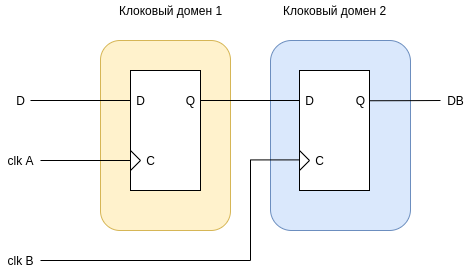
\includegraphics[width=0.7\linewidth]{course-scheme/images/multiclock-domain}
	\caption{Путь домена синхрочастоты}
	\label{fig:multiclock-domain}
\end{figure}


\section{Основные принципы}

При разработке ультисинхрочастотных проектов следует уделять особое внимание стабильности сигнала. Когда сигнал пересекает домен синхрочастоты, то он появляется в новом домене синхрочастоты как асинхронный сигнал и должен быть засинхронизирован.

Синхронизация предотвращает в новом домене синхрочастоты метастабильное состояние первого запоминающего элемента схемы (триггера), и это позволяет в новом домене работать уже со стабильным сигналом.

\textit{Метастабильность} --- это неспособность триггера достигнуть известного состояния в определенный момент времени. Когда триггер входит в метастабильное состояние, то невозможно предсказать ни уровень выходного напряжения элемента, ни период времени, за который этот выход перейдет к правильному уровню напряжения. 

В течение этого переходного времени выход триггера будет находиться на некотором промежуточном уровне напряжения или колебаться и может передать этот недопустимый уровень сигнала со своего выхода к другим триггерам схемы.

\section{Решение проблемы метастабильности}

С целью решения проблемы метастабильности применяются каскады стабилизирующих триггеров, включенных последовательно. Рассмотрим это решение.


Простейший синхронизатор представляет собой два триггера, включенных последовательно без какой-либо комбинационной схемы между ними. Такая схема проекта гарантирует, что первый триггер выходит из своего метастабильного состояния, и его выход переходит в устойчивое состояние перед тем, как второй триггер сохраняет его. Необходимо также разместить эти триггеры, насколько возможно, ближе друг к другу для того, чтобы гарантировать наименьшую расфазировку тактовых сигналов между ними. 

Другой тип ячейки синхронизатора представляет собой два близко расположенных триггера без какой-либо комбинационной логики между ними. Для того чтобы синхронизация работала должным образом, сигнал, пересекающий домен синхрочастоты, должен проследовать от триггера в домене синхрочастоты источника сигнала к первому триггеру синхронизатора, не пройдя через комбинационную логику \ref{fig:sync-triggers}). Схема синхронизации приведена на Рисунке \ref {fig:sync-scheme}.


\begin{figure}
	\centering
	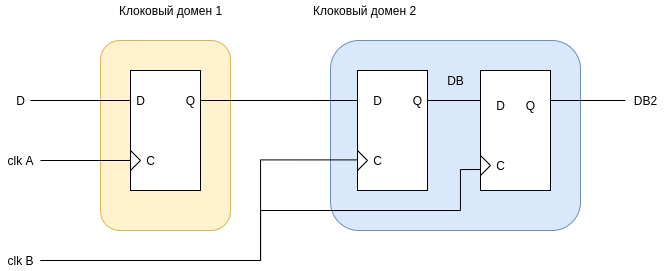
\includegraphics[width=0.7\linewidth]{course-scheme/images/sync-triggers}
	\caption{Триггеры синхронизации}
	\label{fig:sync-triggers}
\end{figure}

\begin{figure}
	\centering
	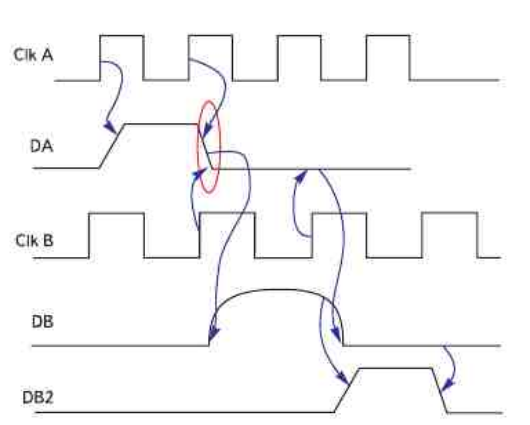
\includegraphics[width=0.5\linewidth]{course-scheme/images/sync-scheme}
	\caption{Схема синхронизации сигнала}
	\label{fig:sync-scheme}
\end{figure}



Данный способ борьбы с метастабильностью будет в дальнейшем использован при разработке узла ресихронизации данных.
